%%
%% BIOTS - Hackathon 2018
%%
%% Roy Schubiger, 2018
%% 
%% Licence: Creative Commons Attribution-Share Alike 3.0 Unported
%% http://creativecommons.org/licenses/by-sa/3.0/
%% 

\documentclass[portrait,a4paper]{article}

\usepackage[utf8x]{inputenc}
\usepackage{amssymb, amsfonts, amsmath}
\usepackage{xcolor}
%\usepackage[e]{esvect}
\usepackage{floatrow} % allows to insert pictures into proofs and theorems

\usepackage{cancel}

\usepackage{graphicx}
%\usepackage{picins}
\usepackage{tabularx}
\usepackage{mwe} % for blindtext and example-image-a in example
\usepackage{wrapfig}
\usepackage{subfigure}
\usepackage{framed}
\colorlet{shadecolor}{orange!15}

\usepackage{geometry}
\geometry{a4paper, left=15mm, right=15mm, top=20mm, bottom=20mm} 

\usepackage{multirow}
\usepackage{multicol}
\columnsep24pt
\columnseprule0.1pt

\renewcommand{\baselinestretch}{1.4}

% hyperref
\usepackage[colorlinks=false,pdfborder = {0 0 0 0}]{hyperref}

\parindent0pt
\setcounter{secnumdepth}{4}

%% Redefine the \paragraph command:
\makeatletter
\renewcommand\paragraph{\@startsection{paragraph}{4}{0mm}%
	{-\baselineskip}%
	{0.5\baselineskip}%
	{\normalfont\bfseries}%
}%
\makeatother 

% algorithms
\usepackage{algorithmic}
\usepackage{algorithm}
\algsetup{linenodelimiter=}

% listings
\definecolor{darkgreen}{RGB}{0,127,14}
\usepackage{listings}

\usepackage{listings}
\usepackage{xcolor}
\lstset { %
    language=C,
    backgroundcolor=\color{black!5}, % set backgroundcolor
    basicstyle=\ttfamily\mdseries, % basicstyle=\linespread{5},% basic font setting
    %escapeinside={!}{!},
    tabsize=4,
    morecomment=[l][\color{cyan}]{\#},
    % numbering
    numbers=left, stepnumber=1, numberstyle=\tiny, numbersep=20pt, numberblanklines=false,
    inputencoding=utf8x,
	xleftmargin=30pt,
	xrightmargin=10pt,
	aboveskip=0.5em,
    belowskip=0.5em,
    columns=fullflexible,
	breaklines=true,
	framerule=0mm,
	frame=single,
	showstringspaces=false,
	commentstyle=\color{black!65},	
	captionpos=b,
	float=float,
	mathescape= true,
	columns=fullflexible
}
% theorem package
\usepackage{amsthm}
\usepackage{thmtools}
\newtheoremstyle{my-thm-style}% name
{6pt}% Space above
{5pt}% Space below
{}% Body font
{}% Indent amount
{\bfseries}% Theorem head font
{}% Punctuation after theorem head
{8pt}% Space after theorem head
{}% Theorem head spec (can be left empty, meaning `normal')
\definecolor{orange}{rgb}{1,0.5,0}
\declaretheoremstyle[
headfont=\normalfont\bfseries,
notefont=\mdseries, notebraces={(}{)},
bodyfont=\normalfont,
name={\ignorespaces},
headpunct=,
postheadspace=0pt,
spaceabove=1pt,
mdframed={
  skipabove=2pt,
  skipbelow=2pt,
  hidealllines=false,
  backgroundcolor={orange!40},
  innerleftmargin=8pt,
  innerrightmargin=8pt}
]{box}
\declaretheorem[style=box, numbered=no]{BOX}
\newcommand{\comment}[1]{\begin{BOX} #1 \end{BOX}}

\usepackage[english]{babel} 

\title{bEquality - Automated tracker for gender equality with blockchain \\[-10pt] Creation of an automated and reliable gender equality index}

\author{Lena Csomor, Qianchen Yu, Lena Csomor, Noah Berner, Eric Léger,\\[-4pt] Fredin Thazhathukunnel, Matthias Matti, Lino Telschow, Roy Schubiger}

\date{\today}


\begin{document}

\maketitle

\vspace{1pt}
\hrule
\vspace{1pt}

\begin{center}
	This project has been built in the context of the BIOTS Hackathon 2018\\
	Blockchain and the Internet of Things School\\[8pt]
	\textbf{Project repository:} \url{https://github.com/ETHBiots2018/bEquality}
\end{center}

\vspace{1pt}
\hrule
\vspace{1pt}

\section*{Abstract}

	%introduction
Today, most companies' market value is driven by intangible value,such as reutation or branch equity. Thus, thousands of companies now provide detailed 
extra-financial information. Regulations are mandating increased management disclosure and analysis on sustainability, and investors are analyzing the
comprehensive risks and opportunities of issuers in public and private markets. One aspect of this extra-financial information is data on gender equality.\\
And more and more investors take this data into consideration when investing as research suggests that good gender equality practice can serve as an
indicator for good corporate governance and decision making and these companies might outperform in the future.
%oroblem description
To get a structured, concise and comparable overview of this data, investors often relay on established gender-equality certifications. Unfortunately, this process is costly, time intensive and 	requires multiple revisions to produce reliable data. \footnote{This paragraph is taken from the challenge description handed to us by the UBS}\\

%motivation	
Our project aims to simplify and automate the process of obtaining such a gender-equality certifications based on an existing Gender-Equality-Framework, and to make its results publicly accesible for everybody.\\
%approach
Our approach focuses on the data capture, data storage, data validation and a the display solution of the process.\\
The data is obtained by the means of a website and an app whereas the storage solution relays on an E-voting system, based on the latest blockchain and cryptographic technology. The solution provides the code of the communication interfaces for the website and the app, as well as the necessary code to handle the data for the E-Voting system via blockchain.\\ Furthermore, a Radar-Chart is used to present the results in a straightforward manner.\\

%conclusion	
In conclusion the platform ensures a trustful, transparent and cheap way to create a gender-equality-index, which is useful for people to make investment decisions and for companies to further improve their status with respect to gender equality. % ABSTRACT
	\clearpage
	
	\subsection*{Introduction}
		The current situation of the economy is not fully inclusive for every member of the society, women get discriminated, sexually harassed and do not have equal chance of high salaries and or higher positions in companies.\\
Our Project bEquality aims to punctually recognize inequality by providing a transparent, reliable and efficient gender-equality index for companies. We think that applying and evaluating a gender-equality index should not be expensive and exclusive to companies that can afford it.\\
We aim to improve todays state of society with respect to gender-equality in the economy.\\

This document summarizes our approach to solve this problem. Our solution has come up on a hackathon organized by the Blockchain and Internet of Things School (BIOTS) 2018.\\

We will first present you our whole process systematically and then later dive further into the implementation of the whole process.\\
The reader should have basic programming understanding or basic logical thinking to understand our approach and implementation, we try to explain it as easy as possible.

\comment{
-describe structure of report - done\\
-describe prerequisities - done\\
-general things - Q: what to add more?
}
	
\section{Project}
	
	\subsection{Overview}
		\begin{figure}[H]
	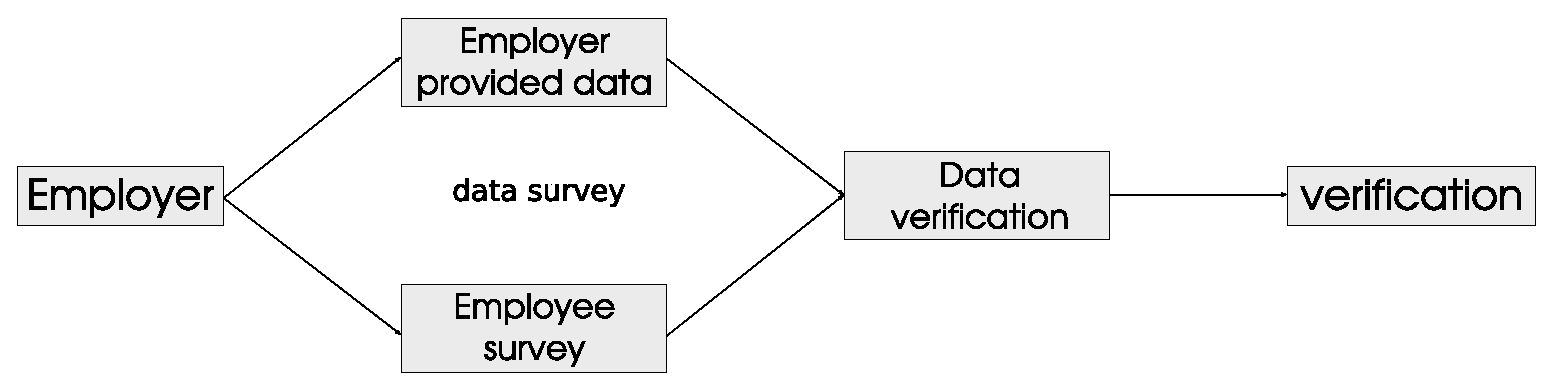
\includegraphics[width=0.9\textwidth]{Bilder/bEquality-project-flow.eps}
	\caption{Project flow graph}
	\label{Project_flow_graph}
\end{figure}
\comment{
-I think the project flow should contain a node for DISPLAY SOLUTION, because this is one of the key points (also one of the points they wanted us to focus on).
-If possible, the texts in the all the nodes should have the same font size
}

The figure \ref{Project_flow_graph} visualizes the high-level structure of our project.\\
Existing gender-equality indices differ from our project at the points \textit{data survey (employee survey)} and \textit{data} \textit{verification} in the high-level structure and in the final evaulation.\\
We will now explain the high-level structure of our project structure.

\paragraph*{Employer Survey}
There are a few necessary steps for an employer to get a certification.
First, the employer has to to send the data asked for by the given rating framework via a Website. Additionaly the company provides the E-mail-Addresses of their employees. That’s the employer provided data.

\comment{Question: do we really take the e-mail addresses?\\
Or does the employer tells every employee to make an account on our platform and then the employer sends us all generated public keys? (sending of public keys can be done implicitly at the registration of the employee) Lena: I think we have to take all email addresses at this point, but we could state it as an unsolved problem since we actually don't want to be a third party etc}

\paragraph*{Employee Survey}
After that, a percentage of employees will be chosen randomly to participate in an employee survey. This survey is used to validate the plausability of the provided data from the employer and to obtain further important private data from employees that cannot be known by the employer.\\

However, this is an easy task for the employee. To set up an account, the employee gets an invitation link from our program and then gets linked to the app, where he/she can set up his/her account. While setting up the account, a public and a private key get generated in the background and linked to the employee account.\\
After the account set-up the company sends all the public-keys generated by the employee account set-up to our framework, this then initiates the survey set-up.\\
When all background work is done, the employee gets a message that the survey is ready. He/she has then just to log into the app, fill out the survey and then submit the data.\\

Everything technical is handled automatically in the background, such that the user just observes a handy interface, and all data is stored on either the blockchain or the IPFS.

\paragraph*{Data Validation}
When all data is gathered from all chosen employees, we split the data into different classes. Either the data from the employees intersect the employer provided data, and is therefore in the \textit{intersecting-data category}, or it is data that is just known or provided by the employee (such as number of sexual harassments or similar things).\\

All data from the \textit{intersecting-data category} gets compared by comparing the provided view of the employer and the view of the employee.\\
This comparison then provides a validity factor for the employer provided data.\\

This process of data validation ensures that the data is not corrupted by either humans or bots.\\

\comment{Q: How is validation done exactly?}

\paragraph*{Display Solution/Evaluation}
We would adapt our evaluation to already existing gender-equality indices. But to further improve these evaluations, we would like to evaluate also different indicators for gender-equality and other measures that are important.\\
\comment { I move this phrase into the Further-points-section, it is too much in the overview: 
And because all the data is digitally available, we could also insert classification via artificial intelligence to even further improve the evaluation process.}
The data evaluation then finally not just results in a single index number, but in a multidimensional spider-diagram, that allows the investor or the company to look closer to existing problems or advantages over the requirement:
\begin{figure}[H]
	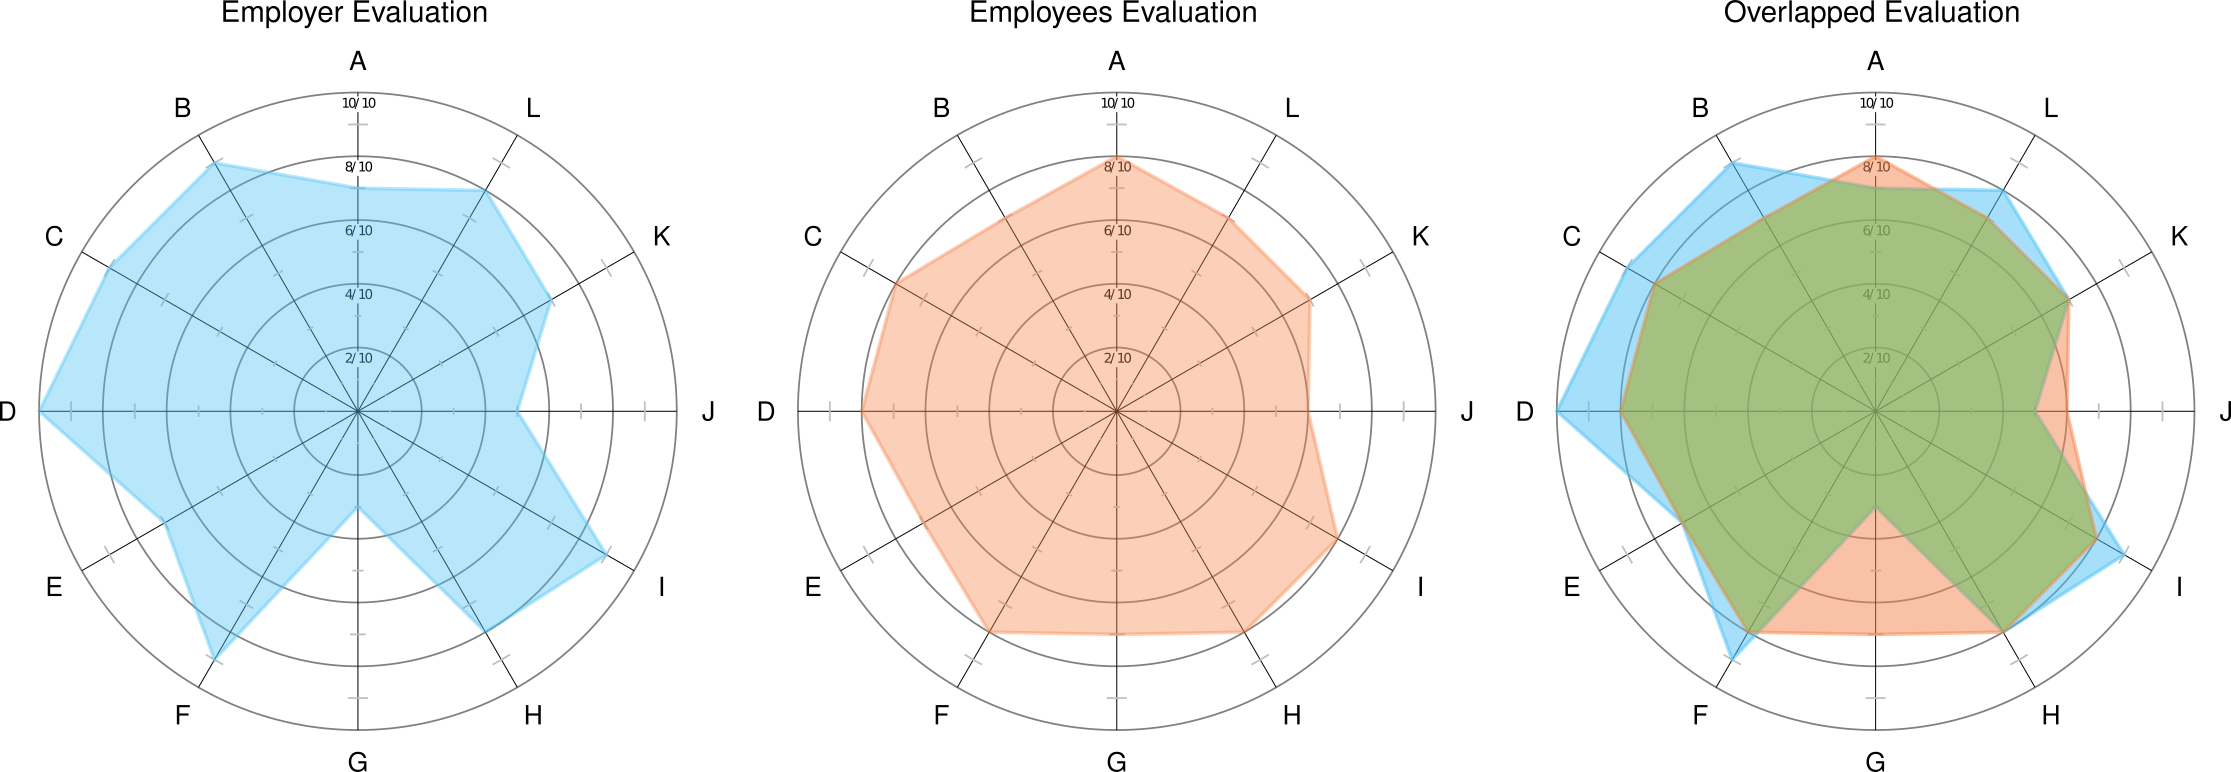
\includegraphics[width=0.95\textwidth]{Bilder/spider-eval}
	\caption{Spider-diagram evaluation example}
	\label{Spider_diagram_evaluation}
\end{figure}
The figure \ref{Spider_diagram_evaluation} provides a flexible evaluation system with detailed feedback.\\
This detailed feedback is useful for company management and also useful for investment decisions by investors that may want to invest in this company. It also implies a feedback system for the company to rate, such that the company knows what to improve in it's employee environment to further improve it's index.
	
	\subsection{Challenges to Solve}
		There are still some challenges to solve for this project.\\[5pt]
One major challenge is to provide a secure way of implementing a system equivalent to E-voting, i.e. to find a system where a user applies to a survey or evaluation and the data provided by him cannot be traced back to this user, even when the user can verify that the data provided by him is used and not some modified version of his data.\\
A way of solving this problem for this use-case (of a gender-equality index) it may be a solution to implement the system in such a way, that cheating for companies are too expensive to be profitable and the company therefore acts cooperatively and provides true data.\\[5pt]
Once we are certain that the company does not cheat we have to look at the behaviour of those who can have a great impact on the evaluation: the employees.\\
We have to assume that the participation rate of the employee survey is rather low, surely not more than 50 percent. This is because people who are moderately happy often do not feel like they have to praise their employer, but they also do not complain. Therefore, most of the people who will respond are either unhappy or very happy, the votes of the moderate people get lost. To get a useful a participation rate, this means we have to send emails to every employee.\\
We have to be certain that with our questions, we get the information we really want. They have to be detailed and unambiguous. Furthermore, we have to adapt the questions for different hierarchy levels. A manager may have other concerns than a worker.
To not lose the participator?s interest, we have to make sure that the questions are short, easy to understand and that there are not too many of them.\\
Also, it is our concern that there is no (easy) way to identify the voter by his answer. A rather simple way to avoid part of it is the strategy of randomised response. This means that if two people are at the exact same point in the survey, let?s say they both have two choices to tick, one may be asked a trivial question, like which sort of ice cream he likes. The other one will be asked a serious question which is important for out data collection. This way, even if someone knows at which point which choice has been made, (for example he sees the employee ticking on his smartphone, but cannot read the question from a distance) he does not know what it meant.\\
We know that anonymising data opens the door for abusers who try to manipulate the survey. The more anonymous the participation is, the easier it is to abuse it. Sadly we have not yet found a way to fix this completely - we can only agree on a certain balance between control and anonymity.\\

	
\comment{
challenges for implementation\\		
-Finding a secure way of implementing a system equivalent to E-voting.\\ 
-Making cheating for companies too hard to be profitable.\\
-privacy for gathering data, boss should not have possibility to see results from its employees\\
-costs\\
Lena: I've added the things I learned from the interview with Prof. Renate Schubert in this section\\
But how do i fix this: participator?s\\

done???
}
			
\section{Technical Implementation}
	
	\subsection{Data Capture and Storage}
		\paragraph*{Company Provided Data}
As already mentioned earlier, the \textit{data capture} process is split into two parts.\\
The first part consists of a survey that is sent to and filled out by the human resources department of the company, i.e. the \textit{company provided data}.\\
The questions on this survey will be based on already existing indices, such as the ones from Bloomberg or Equileap.\\
They fill out the survey directly on the website which stores the data on the blockchain via IPFS. Because the data is stored directly on the blockchain, it is visible for everyone and cannot be tempered with in any way at a later point in time.\\
The company also sends us the email addresses of all their employees, which we will store on a private and secure database. The email addresses can obviously not be stored on the blockchain for privacy reasons. This is a tradeoff in transparency that was inevitable.\\

\paragraph*{Employee Survey}
\comment{The employees will now all get an email and not just a percentage of them.\\
This is  done due to the new insight through the interview, where it is suggested that we use all employees for the survey, because a lot of them wont sign up anyway which will lead to a percentage of employees anyways.}
The second part of \textit{data capture}, the \textit{employee survey}, is a special point of interest. Because it is important to guarantee anonymity to the employee and at the same time ensure validity and transparency of the data that is provided.\\

The first step in the \textit{employee survey} takes part after we received all the email addresses of the employees. We send them an email in which there is a link to our survey app.\\
In the app, they enter a password for a new Ethereum blockchain account which gets generated automatically. The private key of the account is stored only on the employees device and is secured by the password they entered. The app sends the public address of the blockchain to our server, where it is used to load a small amount of Ether onto it. This is done, so that the employee can later make one transaction on the Ethereum blockchain.\\
Once all the employees (or a big enough percentage) have followed our link and created an account, our server will create a new survey contract on the blockchain.\\

This happens via the following smart contract (contract \texttt{SurveyFactory}), where an array of public addresses and a hash to the location of the addresses in IPFS is required to create a new smart contract of the kind \texttt{Survey}.\\
\begin{lstlisting}
// https://github.com/EriCreator/bEquality/blob/master/Survey.sol
/*	SurveyFactory serves as a hub 
	(deployed on the blockchain upon the launching of bEquality)
	Company can create their own survey by providing a list of permitted user address. */

contract SurveyFactory {
  mapping(uint => address) public SurveyContracts;
  ...
  function createNewSurvey(uint companyID, address[] addressessOfEmployees, string _hashToaddressessOfEmployees) public returns(address newContract)
  {
    require(SurveyContracts[companyID] == 0x0);
    Survey c = new Survey(addressessOfEmployees, _hashToaddressessOfEmployees);
    SurveyContracts[companyID] = c;
    return c;
  }
  ...
 }
\end{lstlisting}
\texttt{SurveyFactory} can be thought of as a container in which all the surveys of the different companies are stored and can be accessed via the unique id of the company.

After the \texttt{Survey} contract is created, the employees are notified that they now can fill out the survey. They log into their account on the app and answer the questions provided by us. This is done via a user-friendly interface.\\
The survey for the employees presents them with gender specific questions and also with questions applicable for both men and women. These questions guarantee further insight into the microclimate of the employees that cannot be obtained by just consulting the company management.\\
When they submit the data, it gets stored on IPFS and the hash is again stored on the blockchain.\\
This is done via the smart contract \texttt{Survey} seen below. It takes a hash to the location of the survey results on IPFS and stores it on the blockchain.\\
\begin{lstlisting}
// https://github.com/EriCreator/bEquality/blob/master/Survey.sol
/*
   Survey is the child contract created by the SurveyFactory where only the permitted user can modify.
*/

contract Survey {
    mapping (address => string) public hashes;
    mapping (address => bool) public isAllowedToSumbitSurvey;
    string hashToaddressessOfEmployees;

    function Survey(address[] addressessOfEmployees, string _hashToaddressessOfEmployees) public {
        hashToaddressessOfEmployees = _hashToaddressessOfEmployees;
        for (uint256 index = 0; index < addressessOfEmployees.length; index++) {
            isAllowedToSumbitSurvey[addressessOfEmployees[index]] = true;
        }
    }

    function submitResults(string myHash) public {
        require(bytes(hashes[msg.sender]).length == 0);
        require(isAllowedToSumbitSurvey[msg.sender]);
        hashes[msg.sender] = myHash;
    }

}
\end{lstlisting}
The contract ensures that only the employees addresses which were submitted on contract creation can submit results. It also ensures that an employee can only submit results once and that he/she can not alter any other results.\\
Because the employee knows his/her own public blockchain address (it is displayed on the app), he/she can easily verify that the data on the blockchain did not get altered by anybody.\\
The employee is also the only person who knows that this public key is associated to him/her. Thus the sensitive data stored publicly on the blockchain still insures the privacy of the employee and the employer cannot prosecute the employee for telling his opinion on the company.\\

Below the full protocol is shown in a schematic way, to give the reader an overeview of our E-voting protocol.
\begin{figure}[H]
	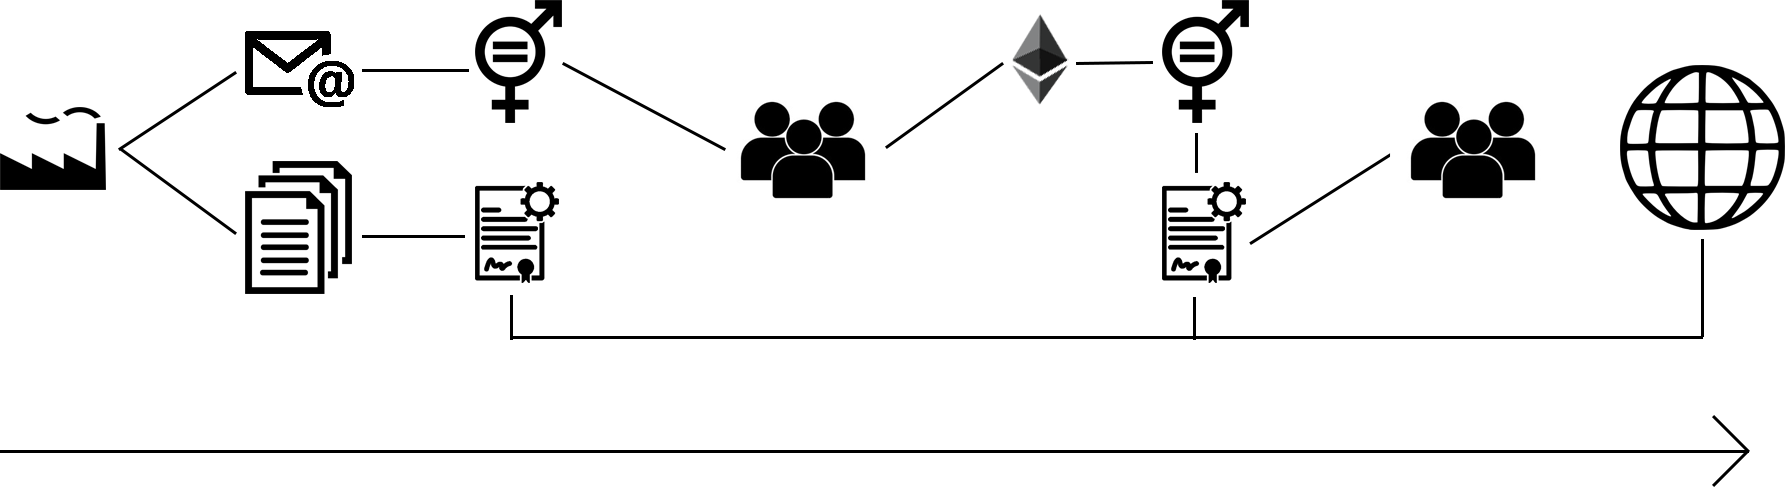
\includegraphics[width=0.9\textwidth]{Bilder/Survey_Protocol_preview_2}
	\caption{technical flow representation of the data capture and storage process}
	\label{technical_flow_representation}
\end{figure}

In our implementation most of the data that gets collected is only stored indirectly on the blockchain via IPFS hashes. This was necessary to reduce the costs of the individual transactions and for overall scalability.\\
Ethereum transaction costs depend, among other things, on the size of the data stored on the blockchain. If we only store hashes instead of survey data, the size of the transaction remains small, no matter the number of questions in the survey.\\

There are still challenges ahead of us for improving our implementation. For example the possibility of storing the public Ethereum addresses on the blockchain instead of a private database while they are still being collected for further transparency and automation of the process.\\

\paragraph*{App Implementation}
To make the survey as easy as possible for the employees, we decided to use an app. We built a demo app for Android smartphones with the Android Studio IDE.\\
The app is only a concept and should serve as a visual guide of how the actual working app would look like. Our demo app consists of a sample survey and dummy buttons and cannot actually submit the survey to the blockchain.\\
Because of the limited time, we were not able to build a working app. Besides the time factor, we did not know how to link the app with the Blockchain/IPFS and if there even is a Java interface to accomplish this task.\\
Nevertheless, our app serves as a great visual reference.\\

\comment{Do not insert pictures as there is a limit of 3 figures in the whole report:
(--insert pictures of the app--)}

The fully implemented app could then work as follows:\\
1. The employee sees a login screen and is asked to fill in his password for the Ethereum blockchain account.\\
2. Once logged in, the app shows the user the questions to answer. The interface is straightforward and self-explanatory.\\
3. After the user submits the survey, the app sends the survey results to the Blockchain/IPFS and reports that the submission was successfull. It also shows the employee his/her blockchain address for verification purposes.\\

The big advantage of an app is the self explanatory user interface.\\

Some of the disadvantages of using an app to collect data are:\\
- Even for one survey, the app needs to be installed on the phones of the employees.\\
- Survey questions are hard-coded into the current app.\\
The second problem can be solved by downloading the questions from a server after the user is logged in. With this approach the app serves as a framework for all kinds of surveys.\\

It is unforeseeable if the app is the right choice to use for the gender equality survey and a good way to find out if it is, would be to test multiple different ways of collecting data and then analysing their effectiveness.\\
				
	\subsection{Data Verification}
		why 2 surveys?:\\
-gives company less chances to actualy deliver wrong information\\
-how is the verification done\\
-After the data verification and evaluation, the evaluated data is stored on IPFS:\\
-Explain the different szenarios: What if.. 
              > Company CEO tries to fill in all the surveys himself?
              > We try to fill in the survey for the company?
              > A few employees try to rate the company baldy?
              ... there may also be some other ones?

		
	\subsection{Display Solution/Evaluation}
		-introduction about this section
-evaluate data and storeed on IPFS:\\
-link evaluated data from IPFS to an App/Web where it is openly accessible
\paragraph*{Multidimensional Approach}

\comment{-----------insert picture of spiderweb here}

-explain display solution with spiderweb\\
-link of emplyer, employee survey and overlapped survey\\
-what can be learned with that\\
-data connected with respective data on IPFS, blockchain\\
-open accessible for everybody\\
-give an example for an indicator an how it could be represented on spider chart ( difference between salaries of men an women).\\
-explain advantages over existing indices\\
--better and clearer view, straightforward\\
--multidimensionality gives a broader picture than just a number\\
-explain challenges and limitations of the spiderweb\\
--which indicators can be displayed, which not\\
					
	\subsection{OTHER THINGS TO ADD HERE}
		todo\\
	\subsection{Further Points Worth to Consider}
		-write about problems that we think that are important, but we didn't have time to consider, or which were to complicated to solve in such a short time\\
-example: which indicators are best to display in Radar-Chart-Diagram, when is a company considered as a Gender-Equal-Company. How should this be measured, how should different companies best be compared...
	

\section{Conclusion}
	\paragraph*{Strengths}
-Our solution provides a reliable, transparent and automatic way of creating a gender-equality index. Compared to other already existing indexes we offer an index where the reliability and correctness can be verified by each and every person. This is done by implementing our strategy on the block-chain. 
-Our approach allows everybody to classify companies according to the latest law regulatory for gender-equality in companies.\\
%strengths/what is working in our solution
-Our solution is multidimensional, where multidimensional stands for two different things. First of all our index contains different categories where the result is weighted and then demonstrated as a graph [graph bild]. The other multidimensionality of our project is that we collect data from two different sources. We collect it from the managers and we collect the data from a casual worker as well.
-public\\
-cheap\\ Nowadays these indexes require a lot of work e.g. to collect the data, to evaluate the data, to present the data in a meaningful way and so on. In our solution we are trying to do as much as possible in an automatic approach.

\paragraph*{Weaknesses}
- Each participant needs to create his own blockchain account before taking the survey\\
- One has to handle a large chunk of data.

\paragraph*{Open Challenges}
There are several ways to expand our project. Examples would be
-to achieve a full working automatic way of indexing gender-equality. This is our main idea but we haven't completed the implementation. The application we use to do the survey has just an interface. This means that we should collect the data on the application and try to put the collected data onto the block-chain for further calculation processes. 
-E-voting system should be improved\\

	
\paragraph*{Disruptional Potential}
-transparency\\
-further enhance gender equality
	

\section{Sources and Literature}

	Sources
In order to develop the app we used:
\begin{itemize}
\item https://developer.android.com
\item https://stackoverflow.com

\end{itemize}

 	Dateiname - Author - Jahr - Link/Buch\\
		
	


% fill the page
\clearpage

%\end{multicols}

\end{document}


